\subsection{El axioma de las paralelas}

El quinto postulado de la geometría de los \textit{Elementos} ha sido crucial en
el estudio de la geometría. Empecemos definiendo el concepto de \textit{líneas
	paralelas} y enunciando el axioma.

\begin{defin*}[Líneas paralelas]
	Se dice que dos líneas $l$ y $m$ son \textbf{paralelas} si no tienen ningún
	punto en común.
\end{defin*}

Una de las formas equivalentes en las que se puede enunciar el axioma de las
paralelas es la siguiente:

\lstleanfull{parallels_independence.lean}{6}{7}

\begin{axb}[P]\label{ax:P}
	Dada una línea $l$ y un punto $A$ existe una única línea $m$ que pasa por
	$A$ y es paralela a $l$.
\end{axb}

\lstleanfull{parallels_independence.lean}{11}{12}

La cuestión principal a determinar, que ha sido un problema abierto durante
varios siglos, hasta la solución del problema en el siglo diecinueve con el
desarrollo de las geometrías no euclídeas, es si el axioma de las paralelas
puede deducirse a partir de los otros axiomas. Es decir, ¿es posible prescindir
del quinto postulado de \textit{Euclides}?

En lógica moderna llamos a esta idea \textit{independencia}. Si no existe forma
de derivar una fórmula dada de un conjunto de fórmulas, decimos que nuestra
fórmula es independiente del resto.

Fijados unos axiomas, decir que una proposición es independiente de ellos
equivale a decir que incluyendo su negación como axioma
obtenemos una teoría consistente, en la que no se pueden demostrar
contradicciones. Esta noción, expresada en términos sintácticos, tiene su
equivalente semántico. Si fijados unos axiomas axiomas podemos construir un
modelo en el que se cumple la proposición y otro en el que se cumple su
contradicción.

Diversos libros modernos de geoemtría euclídea axiomática llaman al conjunto de
axiomas que hemos presentado hasta ahora \textit{planos de Hilbert} (los modelos
de esta teoría reciben el mismo nombre). En esta teoría se cumplen los axiomas
de incidencia, orden y congruencia, pero no se establece el axioma de las
paralelas. Con estos términos, decir que el axioma de las paralelas es
independiente del resto de axiomas equivale a decir que existen planos de
Hilbert en los que se cumple el axioma y otros en los que se cumple su negación.

Con el siguiente teorema hemos formalizado esta idea:

\lstleanfull{parallels_independence.lean}{128}{130}

Usando la táctica \lstinline{push_neg} modificamos la meta inicial a
\lstinline{
	⊢ ∃ cg : congruence_geometry Point Line, ¬ @P Point Line cg.to_incidence_geometry
}.


Una forma de demostrar este resultado es por tanto construyendo un término de
tipo \lstinline{cg : congruence_geometry Point Line} para el cual no se cumpla
el axioma \lstinline{P}.
Para construir dicho término habría que definir una instancia de la clase
\lstinline{congruence_geometry}. Se puede observar por tanto un paralelismo
entre instancias de clases y modelos de teorías.

Algunos modelos simples de planos euclídeos donde no se cumple el axioma de las
paralelas son el \textit{disco de Poincaré} y el \textit{disco de Beltrami}.

\begin{figure}[htbp]
	\centerline{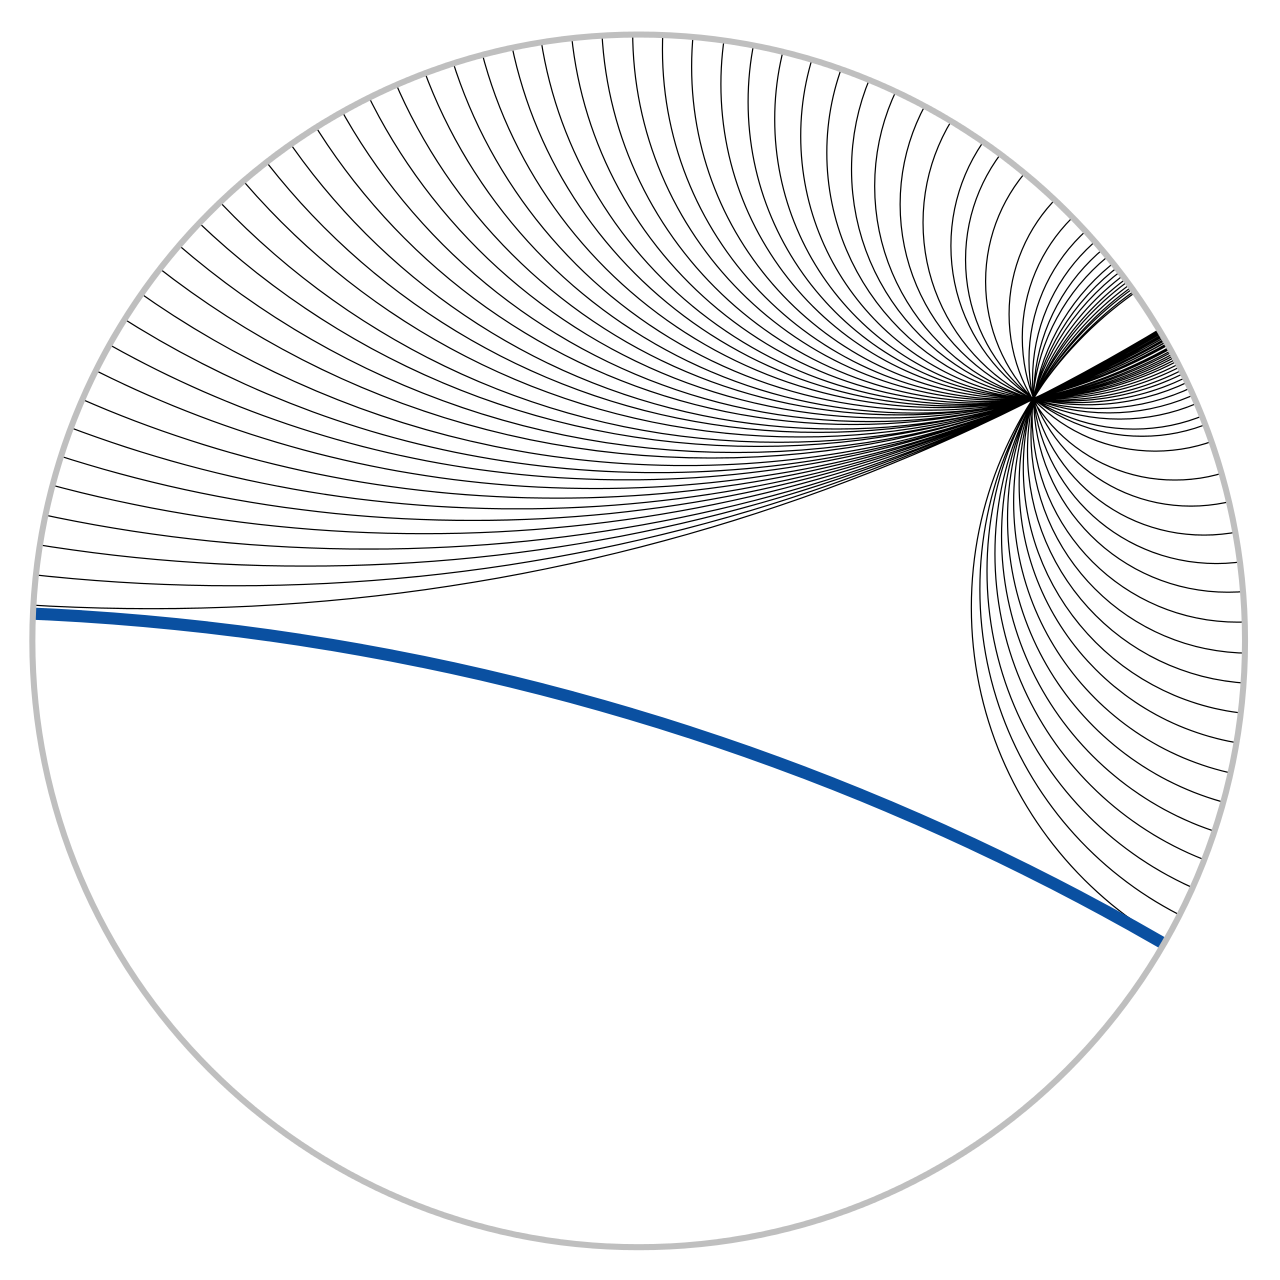
\includegraphics[width=5.5cm]{./imgs/Poincare_disc_hyperbolic_parallel_lines.png}}
	\caption*{En el disco de Poincaré existen infinitas líneas paralelas a una
		dada que pasan por un punto fijo.}
	\label{figure:poincare}
\end{figure}

Podríamos considerar estos modelos y formalizar sus construcciones en \textit{Lean}.
Para ello habría que definir los tipos \textit{Line} y \textit{Point}, las
distintas relaciones de incidencia, orden y congruencia para estos tipos,
demostrar que se cumplen los axiomas de los planos de Hilbert pero no el de las
paralelas. Esto se puede hacer precisamente mediante el mecanismo de las
instancias de clases.








